\documentclass{ximera}

\graphicspath{{./content/02_7_tnb_frames/graphics/}{./graphics/}}

\title{Defining the Moving Frame}
\begin{document}
\begin{abstract}
\end{abstract}
\maketitle

In this section, we introduce the moving frame of a path in $\mathbb{R}^3$, which is also called the TNB frame. This is a set of three mutually perpendicular unit vectors (an orthonormal set) which provide a consistent reference frame for a particle moving along a path.

Imagine yourself walking around, and think about the following three directions:
\begin{itemize}
\item the direction that you're looking (``ahead''),
\item the direction that your head is pointing (``up''),
\item the direction to your right (``right'').
\end{itemize}
Together, the directions ``ahead,'' ``up,'' and ``right'' define your own, personal reference frame. You can describe locations relative to your reference frame:
\begin{center}
``the classroom is up a floor, three doors ahead, and on the right.'' 
\end{center}
However, relative to the rest of the universe, these directions change as you walk around. If you turn around to face in the opposite direction, ahead and right would be pointing in the opposite directions that they were before. If you fly across the world to Australia, the up direction is now in a different direction. So, this frame of reference is unique to your position, and how you are moving around.

Our goal is to define a similar reference frame for a particle moving along a path in $\mathbb{R}^3$, which will consist of three orthonormal vectors. 

\section*{Defining the moving frame}

Suppose we have a path $\vec{x}(t)$ in $\mathbb{R}^3$, and we want to define a reasonable reference frame for a particle moving along this path, which will consist of three mutually orthogonal unit vectors, hence an orthonormal basis for $\mathbb{R}^3$. We'll construct this reference frame one vector at a time, thinking about how we can encode the motion of a particle along the path.

The first vector of our moving frame will match the ``ahead'' direction of our analogy: we want a vector that tells us the direction in which the particle is moving. Since the velocity vector $\vec{x}'(t)$ points in the direction of instantaneous motion along the path, this gives us the correct direction for our first vector. However, the velocity vector isn't necessarily a unit vector. In order to obtain a unit vector in the same direction as the velocity vector, we divide $\vec{x}'(t)$ by its length, obtaining the \emph{unit tangent vector}:
\[
\vec{T}(t) = \dfrac{\vec{x}'(t)}{\|\vec{x}'(t)\|}.
\]

In the video below, you can see how the unit tangent vector changes as we traverse a curve. Notice that the unit tangent vector is always pointing in the direction of motion.

\youtube{PFYJcjdn35o}

For the second vector of our moving frame, we'd like to give the direction in which a particle moving along the path is turning. This doesn't quite match up with the direction ``right'' from our analogy, since you might be turning to either the left or the right. Thinking back to our definition of curvature, we were able to see how a particle was turning by looking at the change in the unit tangent vector. That is, we considered $\vec{T}'(t)$. As it turns out, $\vec{T}'(t)$ will always be perpendicular to $\vec{T}(t)$.

\begin{proposition}
$\vec{T}'(t)\perp \vec{T}(t)$
\end{proposition}

\begin{proof}
Since $\vec{T}(t)$ is a unit vector, we have
\[
\vec{T}(t)\cdot \vec{T}(t) = \answer{1}
\]
for all $t$. Differentiating both sides of this equation, we have
\[
\frac{d}{dt}(\vec{T}(t)\cdot \vec{T}(t)) = \answer{0}.
\]
Using properties of derivatives, we then have
\[
\vec{T}'(t)\cdot \vec{T}(t) + \vec{T}(t)\cdot \vec{T}'(t)=0,
\]
so
\[
\vec{T}'(t)\cdot \vec{T}(t) = 0.
\]
This means that $T'(t)$ and $T(t)$ are perpendicular for all $t$.
\end{proof}

 Since $\vec{T}'(t)$ will always be perpendicular to $\vec{T}(t)$, it's a great candidate for the second direction in our moving frame. However, $\vec{T}'(t)$ won't always be a unit vector, so we'll need to divide by its length to normalize. This gives us the \emph{unit normal vector},
 \[
 \vec{N}(t) = \dfrac{\vec{T}'(t)}{\|\vec{T}'(t)\|}.
 \]
 
In the video below, you can see how the unit tangent vector and unit normal vector change as we traverse a curve. Notice that the unit normal vector is always perpendicular to the unit tangent vector, and that the unit normal vector points in the direction that we're curving.

\youtube{IRpyE1_YCT8}

Together, the unit tangent vector and unit normal vector span a plane, which we call the \emph{osculating plane}. The osculating circle will always lie in the osculating plane.
 
 So far we have the first two vectors of our moving frame, so we just need to find the third. Let's think about how many potential candidates there are for the last vector in our moving frame.
 
 If we have two orthonormal vectors $\vec{v}_1$ and $\vec{v}_2$ in $\mathbb{R}^3$, how many unit vectors in $\mathbb{R}^3$ are perpendicular to both of these vectors?
 \begin{multipleChoice}
 \choice{0}
 \choice{1}
 \choice[correct]{2}
 \choice{3}
 \choice{infinitely many}
 \end{multipleChoice}
 
 We'll choose the third and final vector $\vec{B}$ in our moving frame so that respects the right hand rule with the first two vectors.
 
That is, if you take your right hand, point your fingers in the direction of $\vec{T}$, and curl your fingers in the direction of $\vec{N}$, then your thumb will be pointing in the direction of $\vec{B}$.

\youtube{7f0JAqyAsnU}

Another way to describe the right hand rule is that if you take your right hand, point your index finger in the direction of $\vec{T}$, and point your middle finger in the direction of $\vec{T}$, then your thumb will be pointing in the direction of $\vec{B}$.

\begin{image}
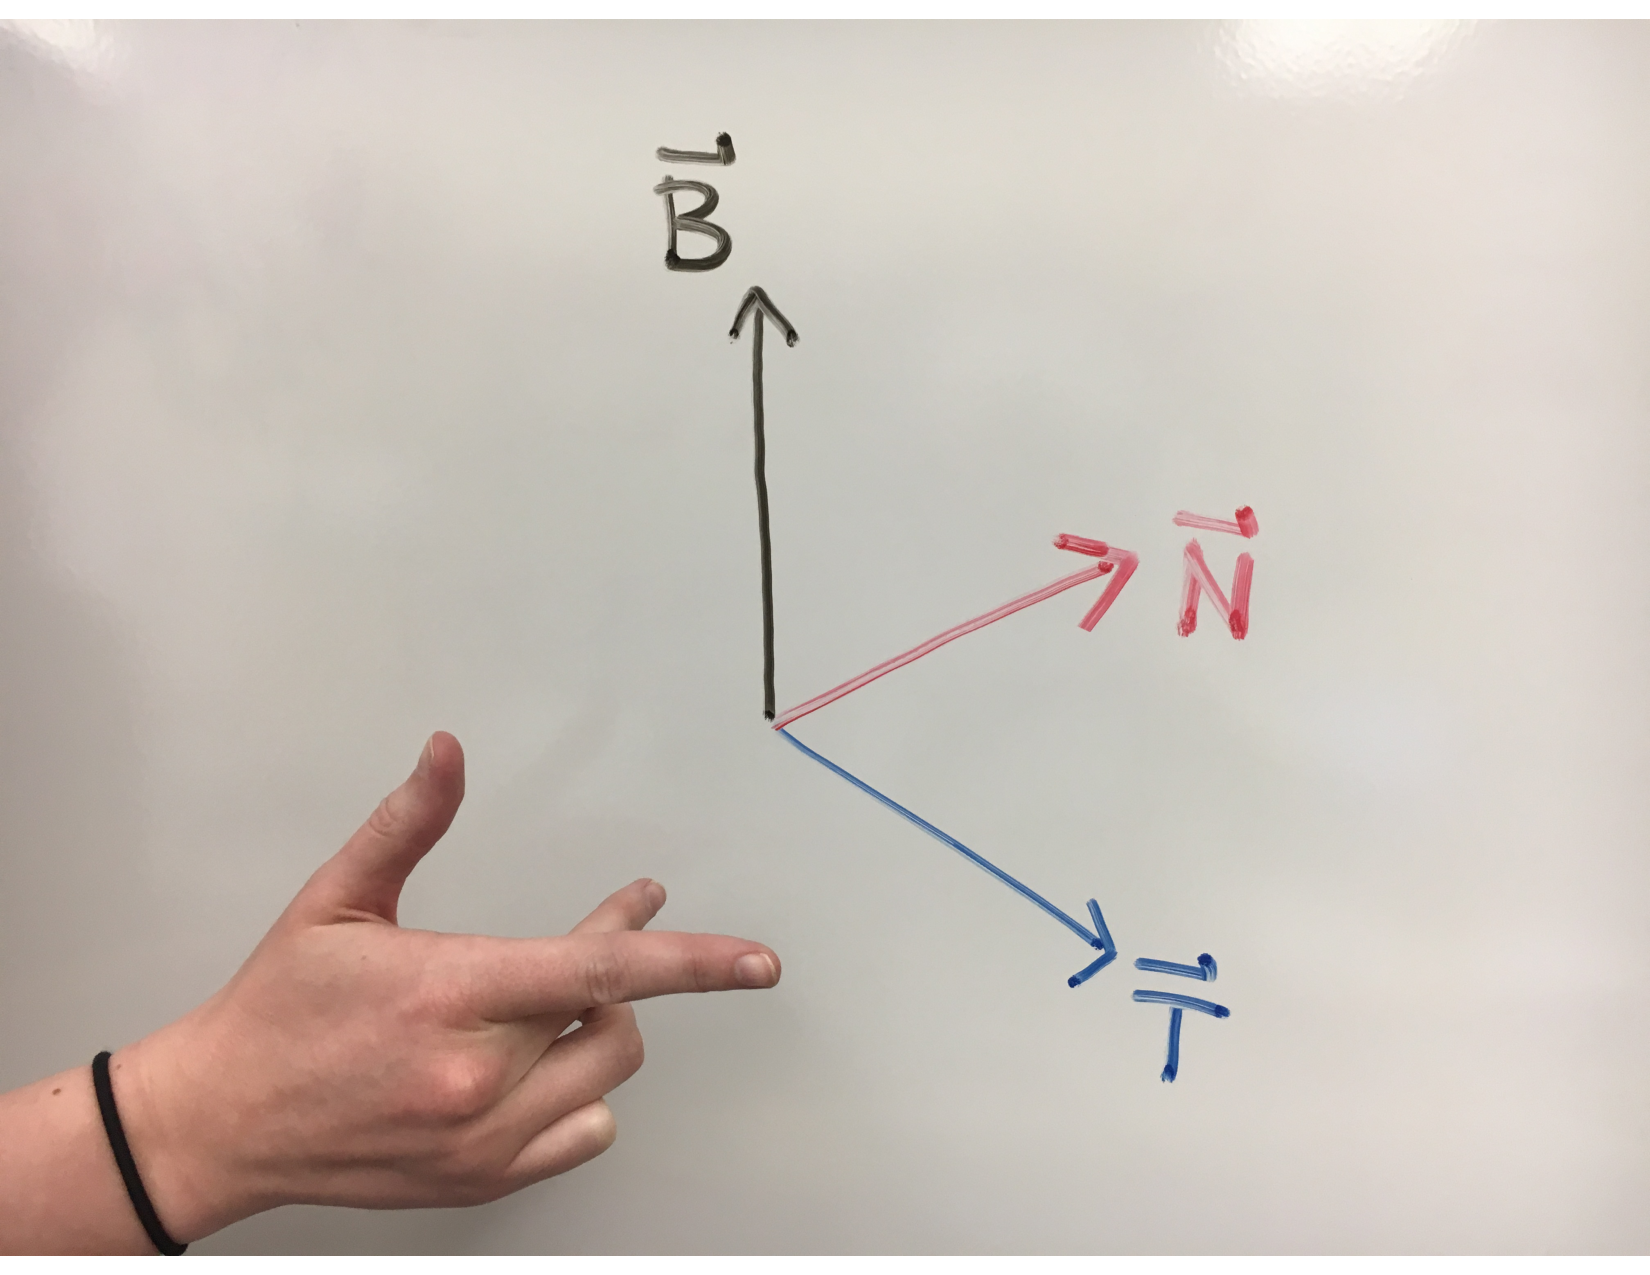
\includegraphics[width = \textwidth]{right_hand_rule}
\end{image}
 
In order to do this, we define the \emph{unit binormal vector} to be
\[
\vec{B}(t) = \vec{T}(t)\times\vec{N}(t).
\]
What is the relationship between $\vec{T}(t)\times\vec{N}(t)$ and $\vec{N}(t)\times\vec{T}(t)$? Select all that apply.
\begin{selectAll}
\choice{They're the same vector.}
\choice[correct]{They have the same length.}
\choice{They point in the same direction.}
\choice[correct]{They point in opposite directions.}
\choice[correct]{One is $-1$ times the other.}
\end{selectAll}
So, we need to be careful about the order of this cross product, so that we choose our unit binormal vector consistently.

Together, $\vec{T}$, $\vec{N}$ and $\vec{B}$ are three mutually perpendicular unit vectors. They form an orthonormal basis for $\mathbb{R}^3$, which changes as we move along the path.

In the video below, you can see how the unit tangent vector, unit normal vector, and unit binormal vector change as we traverse a curve. Notice that the unit binormal is always perpendicular to the unit tangent and unit normal vectors, and that it respects the right hand rule.

\youtube{8sqA5OfrpCQ}

We now summarize the above derivations in our definition of the moving frame.

\begin{definition}
Given a path $\vec{x}(t)$, we define the \emph{moving frame} of the path to be the triple $(\vec{T},\vec{N},\vec{B})$.

$\vec{T}$ is the \emph{unit tangent vector},
\[
\vec{T}(t) = \dfrac{\vec{x}'(t)}{\|\vec{x}'(t)\|}.
\]

$\vec{N}$ is the \emph{unit normal vector},
\[
\vec{N}(t) = \dfrac{\vec{T}'(t)}{\|\vec{T}'(t)\|}.
\]

$\vec{B}$ is the \emph{unit binormal vector},
\[
\vec{B}(t) = \vec{T}(t)\times\vec{N}(t).
\] 

The moving frame is also called the \emph{TNB frame}.
\end{definition}

\textit{Images were generated using \href{https://www.monroecc.edu/faculty/paulseeburger/calcnsf/CalcPlot3D/}{CalcPlot3D}.}

\end{document}